\section{Sprint 1 - Authentication \& Roles Management}

\subsection{Sprint 1 Backlog}

The first sprint focuses on establishing the fundamental authentication infrastructure and user management capabilities for the Credix mobile payment application. This sprint implements role-based access control distinguishing between Corporate Admins and End Users, with automatic wallet creation upon user account setup. The following table presents the user stories prioritized for this sprint:

\begin{table}[!htbp]
  \centering
  \small
  \caption{Sprint 1 Backlog - Authentication \& Roles Management}
  \label{tab:sprint1_backlog}
  \begin{tabular}{|p{1.5cm}|p{3.5cm}|p{7cm}|p{2cm}|}
    \hline
    \textbf{ID} & \textbf{User Story} & \textbf{Description} & \textbf{Priority} \\ \hline
    US1 & Secure Authentication for Corporate Admins  
      & As a corporate admin, I want to authenticate using secure credentials so that I can access the admin dashboard safely and receive a JWT containing my role.  
      & Critical \\ \hline
    US2 & Manage End User Accounts  
      & As a corporate admin, I want to create, update, and delete end user accounts to control who has access to the payment system.  
      & High \\ \hline
    US3 & Secure Authentication for End Users  
      & As an end user, I want to log in with my corporate-provided credentials so that I can access my wallet securely.  
      & High \\ \hline
    US4 & Automatic Wallet Creation  
      & As an end user, I want my wallet to be created automatically upon account creation so that I can start using the payment system immediately.  
      & Medium \\ \hline
  \end{tabular}
\end{table}

\subsection{Use Case Diagram}

The following diagram illustrates the main use cases implemented during Sprint 1, showing the interactions between the Corporate Admin actor and the system functionalities for user and wallet management.

\begin{figure}[H]
  \centering
  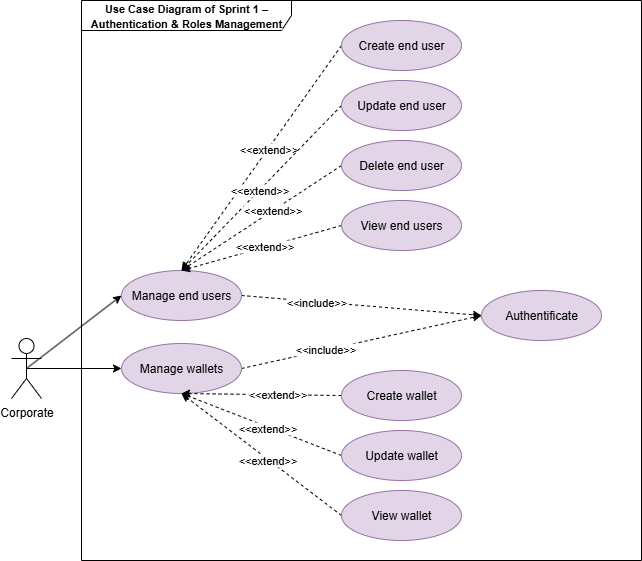
\includegraphics[width=0.75\textwidth]{images/usecase_sprint1.png}
  \caption{Sprint 1 Use Case Diagram - Authentication \& Roles Management}
  \label{fig:sprint1_usecase_diagram}
\end{figure}

\subsection{Detailed Use Case Descriptions}

\subsubsection{UC1: Manage End Users}

\begin{longtable}{|p{4cm}|p{10cm}|}
        \caption{Description of Use Case « Manage End Users »}
  \label{tab:uc_manage_end_users} \\
 \hline
  \textbf{Title} & Manage End Users \\ \hline
  \textbf{Primary Actor} & Corporate Admin \\ \hline
  \textbf{Description} & This use case allows the corporate admin to:
    \begin{itemize}[nosep,leftmargin=*]
      \item create, update, or delete end user accounts;
      \item assign secure login credentials;
      \item enable or disable access to the payment system;
      \item view the list of users and their statuses.
    \end{itemize} \\ \hline
        \textbf{Preconditions} & The corporate admin is authenticated and has the rights to manage user accounts. \\ \hline
    \textbf{Postconditions} & User accounts are created, updated, or deleted; wallets are automatically created for new users. \\ \hline
    \textbf{Nominal Scenario} &
      \begin{enumerate}[nosep,leftmargin=*]
        \item The admin accesses the user management interface.
        \item The system displays the list of existing accounts with their statuses.
        \item The admin chooses to add, modify, or delete an account.
        \item The admin enters or modifies account information (email, password, role).
        \item The system validates the data and records the modification.
        \item For a new user, the system automatically creates a wallet.
        \item The system confirms the update of user accounts.
      \end{enumerate} \\ \hline
    \textbf{Alternative Scenarios} &
      \begin{enumerate}[nosep,leftmargin=*]
        \item If a required field is empty, the system displays « Required Field » and blocks the action.
        \item If the email already exists, the system displays « User already exists ».
        \item If the admin cancels the action, no modification is made.
      \end{enumerate} \\ \hline
    \textbf{Exception Scenarios} &
      \begin{enumerate}[nosep,leftmargin=*]
        \item In case of server error or database issue, the system displays « Internal error, please try again ».
      \end{enumerate} \\ \hline
\end{longtable}

\subsubsection{UC2: Manage Wallets}

\begin{longtable}{|p{4cm}|p{10cm}|}
      \caption{Description of Use Case « Manage Wallets »}
  \label{tab:uc_manage_wallets} \\
  \hline
  \textbf{Title} & Manage Wallets \\ \hline
  \textbf{Primary Actor} & Corporate Admin \\ \hline
  \textbf{Description} & This use case allows the corporate admin to create, view, and modify end user wallets. \\ \hline
  \textbf{Preconditions} & The admin is authenticated and has the right to manage wallets. \\ \hline
\textbf{Postconditions} & The wallet is created, updated, or viewed, and its status is updated in the system. \\ \hline
  \textbf{Nominal Scenario} &
    \begin{enumerate}[nosep,leftmargin=*]
      \item The admin navigates to the wallet management interface.
      \item The admin selects a user and chooses « Create », « Update » or « View ».
      \item The admin enters or modifies wallet details (initial balance, status).
      \item The system generates a unique tokenizedId for the new wallet.
      \item The system records the wallet and displays a success message.
    \end{enumerate} \\ \hline
  \textbf{Alternative Scenarios} &
    \begin{enumerate}[nosep,leftmargin=*]
      \item If the user already has a wallet, the system displays « Wallet already exists ».
      \item If the admin cancels the action, the wallet remains unchanged.
    \end{enumerate} \\ \hline
  \textbf{Exception Scenarios} &
    \begin{enumerate}[nosep,leftmargin=*]
      \item In case of tokenizedId generation failure, the system displays « Wallet creation error ».
    \end{enumerate} \\ \hline
\end{longtable}

\subsubsection{UC3: Authenticate}

\begin{longtable}{|p{4cm}|p{10cm}|}
      \caption{Description of Use Case « Authenticate »}
  \label{tab:uc_authenticate} \\
  \hline
  \textbf{Title} & Authenticate \\ \hline
  \textbf{Primary Actor} & End User / Corporate Admin \\ \hline
  \textbf{Description} & This use case allows users to authenticate into the system with their credentials to access appropriate functionalities based on their role. \\ \hline
  \textbf{Preconditions} & The user has valid credentials and the application is accessible. \\ \hline
\textbf{Postconditions} & The user is authenticated, receives a JWT token, and accesses the role-appropriate interface. \\ \hline
  \textbf{Nominal Scenario} &
    \begin{enumerate}[nosep,leftmargin=*]
      \item The user opens the application and sees the login interface.
      \item The user enters their email and password.
      \item The system validates the credentials against the database.
      \item The system generates a JWT token containing role information.
      \item The user is redirected to the appropriate interface (admin dashboard or user wallet).
    \end{enumerate} \\ \hline
  \textbf{Alternative Scenarios} &
    \begin{enumerate}[nosep,leftmargin=*]
      \item If the user chooses « Remember me », the token is securely stored locally.
      \item If it's the first login, the system may prompt for additional setup.
    \end{enumerate} \\ \hline
  \textbf{Exception Scenarios} &
    \begin{enumerate}[nosep,leftmargin=*]
      \item If the credentials are invalid, the system displays « Invalid email or password ».
      \item If the account is deactivated, the system displays « Account suspended, contact admin ».
      \item In case of network error, the system displays a connection error with retry option.
    \end{enumerate} \\ \hline
\end{longtable}

\subsection{Sequence Diagrams}

The following sequence diagrams illustrate the main interactions between different actors and system components for the key use cases of Sprint 1. Each diagram shows the detailed flow of operations for authentication and user management processes.

\subsubsection{Authentication Sequence Diagram}

This diagram illustrates the authentication process where a user (either end user or corporate admin) enters their credentials. The authentication interface transmits this information to the authentication controller, which validates credentials through the user service against the database. Upon successful validation, a JWT token is generated and returned; otherwise, an error message is displayed.

\begin{figure}[H]
\centering
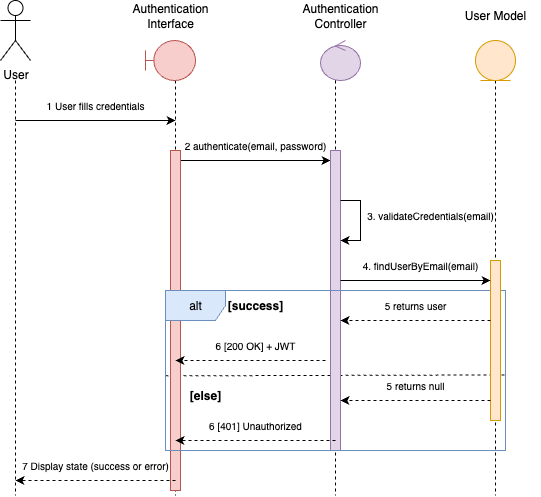
\includegraphics[width=0.9\textwidth]{images/seq_authentication.png}
\caption{Authentication Sequence Diagram}
\label{fig:seq_authentication}
\end{figure}

\subsubsection{User Creation Sequence Diagram}

This diagram shows the user creation process initiated by a corporate admin. The admin submits user details through the interface, which are processed by the user controller and service. The system validates the data, checks for existing users, creates the new user account, and automatically triggers wallet creation for the new user.

\begin{figure}[H]
\centering
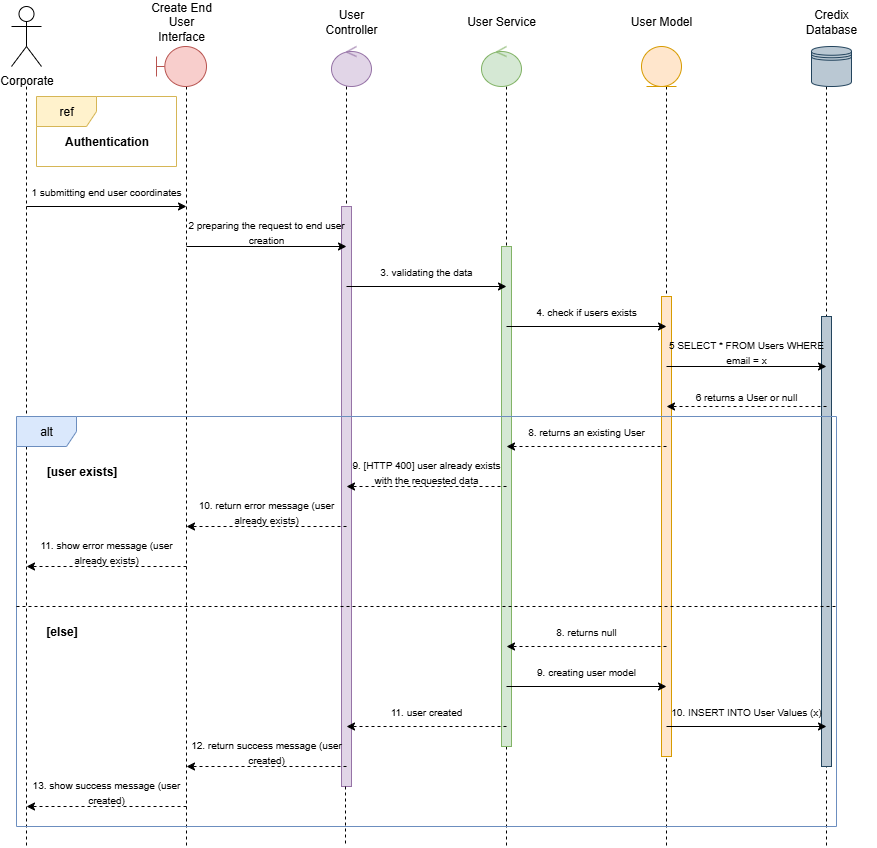
\includegraphics[width=0.9\textwidth]{images/seq_user_creation.png}
\caption{User Creation Sequence Diagram}
\label{fig:seq_user_creation}
\end{figure}

\subsection{Class Diagram (Sprint 1)}

The Sprint 1 class diagram, presented in Figure~\ref{fig:class_sprint1}, establishes the foundational business entities and their relationships:

\begin{itemize}[nosep,leftmargin=*]
\item \textbf{User}: Base entity with email, password, and timestamps
\item \textbf{Admin}: Inherits from User, represents corporate administrators
\item \textbf{End User}: Inherits from User, represents wallet owners
\item \textbf{Corporate}: Entity representing the corporate organization
\item \textbf{Wallet}: Digital wallet with tokenizedId, balance, and status
\end{itemize}

The diagram shows inheritance relationships between User and its subclasses (Admin, End User), as well as the association between Corporate and End User entities. Each End User owns exactly one Wallet, establishing a one-to-one relationship.

\begin{figure}[H]
\centering
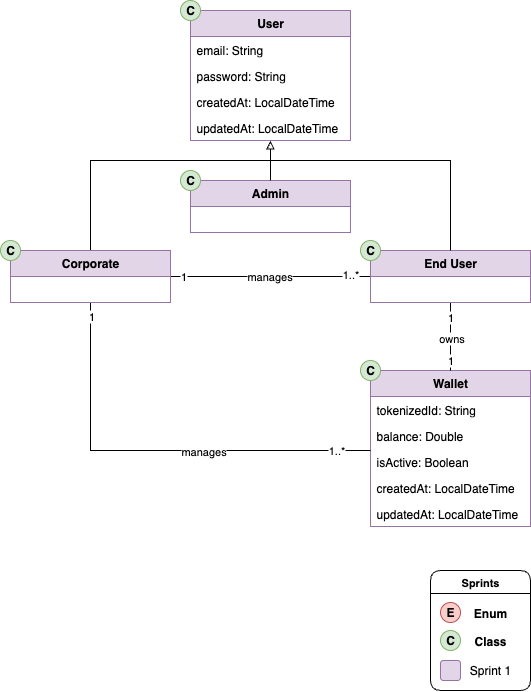
\includegraphics[width=0.9\textwidth]{images/class_sprint1.png}
\caption{Class Diagram - Sprint 1}
\label{fig:class_sprint1}
\end{figure}

\subsection{Implementation (Sprint 1)}

In this section, we present the main interfaces developed during Sprint 1, focused on secure authentication and user management. The implementation covers both mobile application interfaces for end users and web dashboard interfaces for corporate administrators.

\subsubsection{Authentication Interface}

The login interface provides secure access for both end users and corporate administrators. The interface adapts based on user role, redirecting to appropriate dashboards upon successful authentication.

— \textbf{Key Features:}
\begin{itemize}[nosep,leftmargin=*,label=•]
\item Email and password input fields with validation
\item Role-based redirection (admin dashboard vs user wallet)
\item JWT token generation and secure storage
\item Error handling for invalid credentials and network issues
\end{itemize}

— \textbf{Authentication Flow:}
\begin{itemize}[nosep,leftmargin=*,label=•]
\item User enters credentials and submits login form
\item System validates against user database with encrypted password comparison
\item On success: JWT token generated and user redirected to role-appropriate interface
\item On failure: Clear error message displayed with retry option
\end{itemize}

\subsubsection{Corporate Admin Dashboard}

The web-based admin dashboard provides comprehensive user and wallet management capabilities for corporate administrators.

— \textbf{Key Features:}
\begin{itemize}[nosep,leftmargin=*,label=•]
\item User management: Create, update, delete, and view end user accounts
\item Wallet management: Create wallets, view balances, and monitor status
\item Bulk operations for efficient user onboarding
\item Audit logging for all administrative actions
\end{itemize}

— \textbf{Admin Workflow:}
\begin{itemize}[nosep,leftmargin=*,label=•]
\item Admin authenticates and accesses management dashboard
\item Creates end user accounts with corporate email addresses
\item System automatically generates wallets for new users
\item Admin can monitor user activity and wallet status
\end{itemize}

\subsubsection{End User Mobile Interface}

The mobile application provides end users with secure access to their wallet information and basic account management.

— \textbf{Key Features:}
\begin{itemize}[nosep,leftmargin=*,label=•]
\item Secure login with corporate credentials
\item Wallet balance display and account information
\item Profile management and security settings
\item Responsive design optimized for mobile devices
\end{itemize}

— \textbf{User Experience:}
\begin{itemize}[nosep,leftmargin=*,label=•]
\item Simple, intuitive login process
\item Immediate access to wallet information post-authentication
\item Clear navigation and user-friendly interface design
\item Secure session management with automatic logout
\end{itemize}
